\begin{table}[htbp]
	\centering
	\caption{List of measurement equipment and components}\label{tab_appendix:KtSetUp}
	
	\begin{tabularx}{\textwidth}{lXXXX}
		Name 				& Brand	& Model & AAU-number									\\ \toprule \rowcolor{lightGrey}
		Oscilloscope	& Agilent & 54621D & 33941 	\\
		Powersupply	& Agilent & E3631A & 78577\\ \rowcolor{lightGrey}
		DC motor & Alsthom BBC & F9M2& 08339
	\end{tabularx}
\end{table}

\subsubsection*{Setup}
\autoref{fig:KtMeasurementSetup} shows a diagram and photo of the measurement set up
\begin{figure}[htbp]
	\centering
	\begin{subfigure}{0.50\textwidth}
			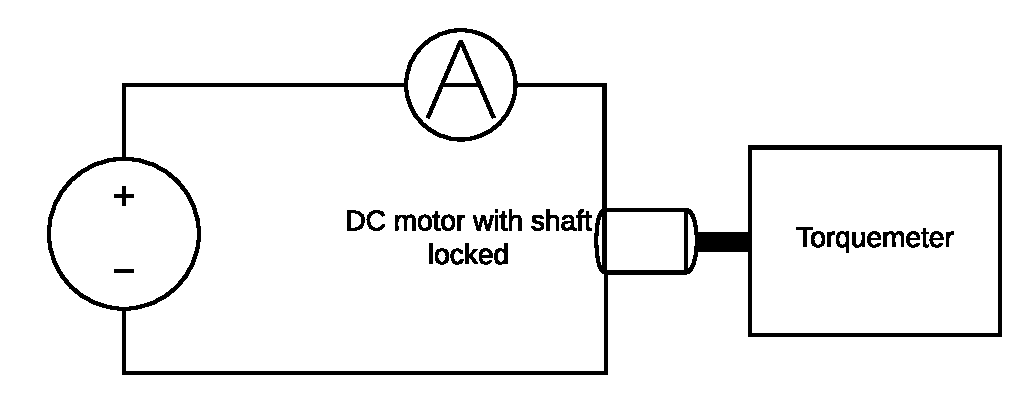
\includegraphics[width=\textwidth]{KtTestSetUp}
		\caption{Diagram of the setup.} \label{fig:KtMeasurementDiagram}
	\end{subfigure}
	\begin{subfigure}{0.40\textwidth}
		%\includegraphics[width=1\textwidth]{MotorImpedanceTest.jpg}
		\missingfigure{Picture of the setup}
		\caption{Picture of the setup.} \label{fig:KtMeasurementPictures}
	\end{subfigure}
	\caption{The measurement setup.} \label{fig:KtMeasurementSetup}   
\end{figure}

\subsubsection*{Method}
This test consists of having the motor shaft locked while the torque $\tau_m$ and the current $I$ are measured.
\newpage


\subsubsection*{Raw data}
\autoref{tab_appendix:KtData} has all the measurements done.

\begin{figure}[htbp]
	\centering
	\caption{Raw data used to determine $K_t$}\label{tab_appendix:KtData}
	\begin{tabularx}{0.35\textwidth}{XX}
		Current (I) & $\tau_m$\\ \toprule \rowcolor{lightGrey}
	4.0 & 0.1164 \\
	4.5 & 0.1314 \\ \rowcolor{lightGrey}
	5.0 & 0.1498 \\
	5.5 & 0.1606 \\ \rowcolor{lightGrey}
	6.0 & 0.1824 \\
	6.5 & 0.1896 \\ \rowcolor{lightGrey}
	7.0 & 0.2050 \\
	7.5 & 0.2192 \\ \rowcolor{lightGrey}
	8.0 & 0.2332 \\
	8.5 & 0.2478 \\ \rowcolor{lightGrey}
	9.0 & 0.2604 \\
	9.5 & 0.2750 \\ \rowcolor{lightGrey}
	10.0 & 0.2900
	\end{tabularx}
\end{figure}

\subsubsection*{Data processing}

When the motor is in steady state and the shaft locked as shown in \autoref{fig:KtMeasurementDiagram}, \autoref{eq:KtTest} is found from \autoref{eq:MotorTorque}.

\begin{equation}\label{eq:KtTest}
	K_t=\frac{\tau_m}{I} \addunit{\newton\meter\per\ampere}
\end{equation}

\startexplain
\explain{$I$ is the current in the circuit}{\si{\ampere}}
\explain{$\tau_m$ is the torque of the motor}{\si{\newton\meter}}
\explain{$K_t$ is the motor's torque constant}{\si{\newton\meter\per\ampere}}
\stopexplain

\subsubsection*{Conclusion}

\autoref{fig:KtTest} plot the $K_t$ found for each measurement. The $K_t$ used in the model is average of these points. This gives $K_t=\SI{0.0293}{\newton\meter\per\ampere}$

\begin{figure}[htbp]
	\centering
	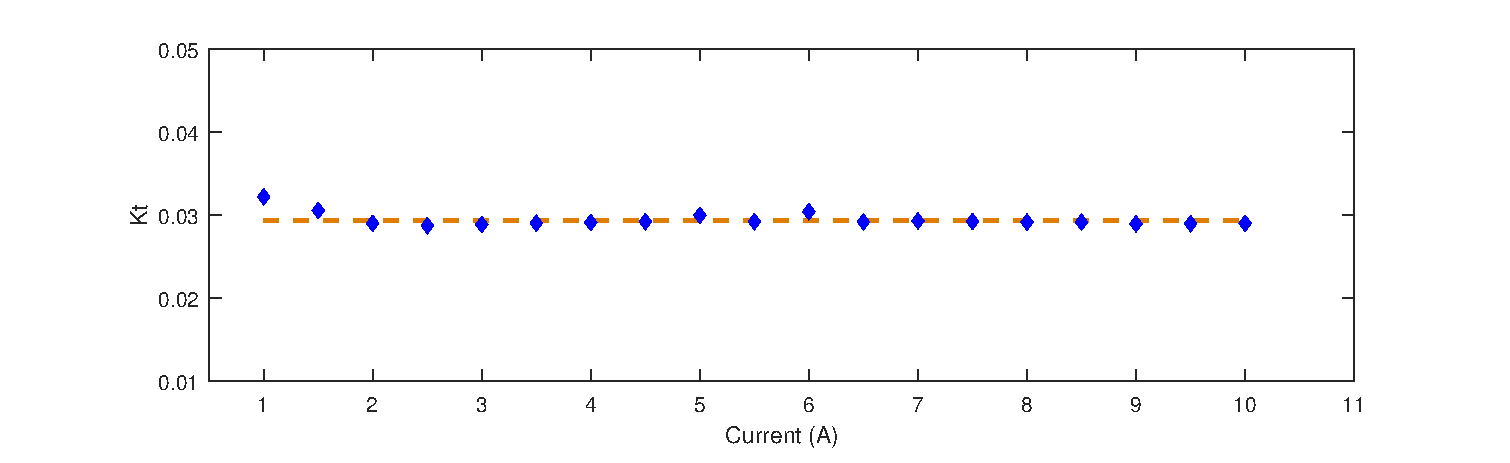
\includegraphics[width=\textwidth]{figures/appendix/Motor&GearTests/PlotKt}
	\caption{Plot of $K_t$ found for each measures}\label{fig:KtTest}
\end{figure}